\documentclass{article}
\usepackage[utf8]{inputenc}

%% Useful packages
\usepackage{helvet}
\renewcommand{\familydefault}{\sfdefault}
\usepackage{hyperref}
\usepackage{amsmath}
\usepackage{siunitx}
\usepackage[margin=1 in]{geometry}
\usepackage{indentfirst}
\usepackage{graphicx}
\usepackage{listings}
\setlength{\parskip}{0.5 em}
\usepackage{tikz}
\usetikzlibrary{shapes.geometric, arrows, decorations.pathreplacing}

\newenvironment{descriptions}
  {\par\vspace{\abovedisplayskip}\begin{tabular}{>{$}r<{$} @{$:{}$} l}}
  {\end{tabular}\par\vspace{\belowdisplayskip}}

\newenvironment{newdescriptions}
  {\begin{tabular}{>{$}r<{$} @{$:{}$} l}}
  {\end{tabular}}

\newcommand{\code}[1]{\texttt{#1}}

\title{An introduction to BioCro for those who want to add models.}
\author{Justin McGrath}

\begin{document}
\maketitle
\section{Plant growth as a system of differential equations}
\subsection{Overview}
BioCro is used to calculate aspects of plant growth, such as the current mass of the plant, given aspects about the plant and its environment that are already known, such as air temperature. For example, one can calculate leaf and stem mass over thermal time given measures of the climate (Figure \ref{fig:example}).
% * <jesse.mcgrath@gmail.com> 2017-07-19T17:37:22.667Z:
% 
% > Leaf and Stem
% lowercase, leaf and stem?
% 
% ^ <mcgrath.justin@gmail.com> 2017-07-21T14:11:10.210Z.

\begin{figure}[!h]
\centering
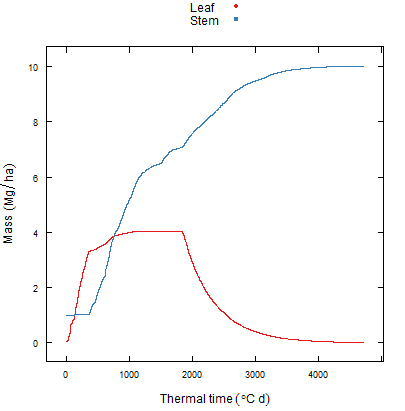
\includegraphics[width=0.3\textwidth]{example_gro.png}
\caption{\label{fig:example}Mass over time of willow.}
\end{figure}

The use of the BioCro is designed to reflect differential equation models. If you're already familiar with such models, skip to section \ref{sec:math_summary}.
% * <jesse.mcgrath@gmail.com> 2017-07-19T17:37:53.099Z:
% 
% > the
% delete "the".  Also the sentence is unusual.  The subject is "use" and verb is "is designed".  "BioCro is designed to reflect differential equation models" is probably better.
% 
% ^.

We'll call the set of all of the variables in the model (mass, temperature, wind speed, etc) the state. We want to calculate the state for some time period: for example, every hour from June 1 to August 1.  We'll denote the state over the whole period as $X$, and the state at a specific time, $t$, as $X_t$.
% * <jesse.mcgrath@gmail.com> 2017-07-19T17:39:55.506Z:
%
% > We'll call the set of all of the variables in the model (mass, temperature, wind speed, etc) the state. We want to calculate the state for some time period: for example, every hour from June 1 to August 1.  We'll denote the state over the whole period as $X$, and the state at a specific time, $t$, as $X_t$.
%
% ^.

Some parts of the state are known \textit{a priori} for the entire period, and we'll denote these as $X_k$ ($k$ for known), and denote the known state at time, $t$, as $X_{t,k}$. These values that are known beforehand are inputs of the model, and in literature, people typically say that these variables "drive" the model.

Some state variables can be calculated from other state variables without explicit dependence on time. For example, the total mass of the plant is the sum of leaf, stem and root masses.  This set of variables we'll denote as $X_{cs}$ ($cs$  for \underline{c}alculated from \underline{s}teady state). 

Some variables must be calculated from the rate of change, and therefore they depend explicitly on time. For example, the rate of change of leaf mass is calculated from the photosynthetic rate, so the leaf mass at 10 am is the leaf mass at 9 am plus the rate of change, times one hour (3600 seconds).  $mass_{10am} = mass_{9am} + \frac{dmass}{dt} * \SI{3600}{s}$. The variables we calculate from rates of change we'll denote as $X_{cd}$ ($cd$ for \underline{c}alculated from \underline{d}ifferential equations).

As with $X$ and $X_t$, to denote a specific time a subscript $t$ is used: for example, $X_{t, cd}$. Since each $X_{t,cd}$ depends on the previous value, that is $X_{t-1, cd}$, the initial value, that is $X_{0, cd}$, must be given as input to the model.

We'll denote the equations that describe how to calculate steady-state variables ($X_{t,cs}$) from variables we know beforehand ($X_{t,k})$ as $g(X_{t,k})$. Thus, $X_{t,cs} = g(X_{t,k})$.
% * <jesse.mcgrath@gmail.com> 2017-07-19T18:21:12.208Z:
% 
% > The equations that describe how to calculate steady-state variables ($X_{t,cs}$) from variables we known beforehand ($X_{t,k})$ we'll denote as $g(X_{t,k})$. Thus, $X_{t,cs} = g(X_{t,k})$.
% We'll denote the equations that describe ... as ... .
% 
% ^ <mcgrath.justin@gmail.com> 2017-07-21T14:14:00.550Z.
% * <jesse.mcgrath@gmail.com> 2017-07-19T18:20:42.176Z:
% 
% >  known
% know
% 
% ^ <mcgrath.justin@gmail.com> 2017-07-21T14:14:07.472Z.

The rate of change of variables we want to calculate over time ($\frac{dX_{t,cd}}{dt}$) can depend on any state variable at the current time ($X_{t}$). The equations that describe how to calculate $\frac{dX_{t,cd}}{dt}$ from $X_{t}$ we'll denote as $h(X_{t})$. Thus, $\frac{dX_{t,cd}}{dt} = h(X_{t})$.

The model is solved by iterating through the following process for each time point:
\begin{center}
\begin{enumerate}
\item Calculate the steady-state equations using the parameters that are already known.
\item Combine the known parameters, steady-state parameters, and parameters that depend on differential equations into one set of parameters that holds all of the state variables.
\item Calculate the rates of change using the differential equations and the state variables
\item Use the rates of change to calculate new values for the parameters that depend on differential equations.
\end{enumerate}
\end{center}

This process is described using mathematical notation in section \ref{sec:math_summary}.

\subsection{Mathematical summary}
\label{sec:math_summary}

\subsubsection{Model inputs}
\label{sec:model_inputs}
The inputs to the model are the following:

\begin{table}[!htbp]
\begin{center}
\begin{descriptions}
	X_k & A set of state key-value pairs for variables that are known for the whole simulation period. \\
	X_{0,cd} & A set of state key-value pairs that are initial values of variables calculated over time. \\
	g(X_{t,k}) & A set of equations describing steady-state processes. \\
	h(X_{t}) & A set of differential equations. \\
\end{descriptions}
\caption{\label{tab:model_inputs}Inputs to the model}
\end{center}
\end{table}

\subsubsection{Model equations}
\label{sec:model_equations}
The model is solved by iterating through the following process for each $t$ starting at $t = 0$:
\begin{align}
\label{eq:solver_loop}
\begin{split}
	X_{t,cs} &= g(X_{t,k}) \\
    X_t &= X_{t,k}  \cup X_{t,cs} \cup X_{t,cd} \\
    \frac{dX_{t,cd}}{dt} &= h(X_{t})  \\
    X_{t+1,cd} &= X_{t} + \frac{dX_{t,cd}}{dt} * \Delta t
\end{split}
\end{align}

\subsection{Relating the mathematics to the code}
\subsubsection{Function inputs}

The \code{Gro()} function accepts four parameters that correspond to the model inputs (Table \ref{tab:model_inputs}). For convenience, $X_k$ is separated into state variables that do or do not vary over the simulation period.
% * <jesse.mcgrath@gmail.com> 2017-07-19T18:23:12.360Z:
% 
% > state
% The conjugation is wrong somewhere. Should this be "states that do or do not..."
% 
% ^ <mcgrath.justin@gmail.com> 2017-07-21T14:14:55.897Z.

\begin{table}[!htbp]
\begin{center}
\begin{tabular}{| r | l |}
	\hline
    \textbf{Gro() input} & \textbf{model equivalent} \\ 
    \hline
    \code{initial\_values} & $X_{0,cd}$ \\ 
    \code{parameters} & $X_k$ that do not vary with time. \\ 
    \code{varying\_parameters} & $X_k$ that do vary with time. \\ 
    \code{modules} & $h(X_{t})$ \\ 
    not currently an input & $g(X_{t,k})$ \\
    \hline
\end{tabular}
\end{center}
\end{table}

State variables are represented as a paired name and value, for example [Leaf, 10]. In programming parlance, this concept is usually called a key-value pair, and here "Leaf" is the key and "10" is the value.  In R, the data types that represent this concept are \code{list} and \code{data.frame}. For example, to specify initial values (that is, $X_{0,cd}$) for stem and leaf biomass, one would use the following:
\lstset{
  xleftmargin=0.05\textwidth, xrightmargin=.2\textwidth
}

\begin{center}
\begin{lstlisting}
# The list() function takes any number of key=value pairs, separated by commas.
> example_initial_values = list(Stem = 3, Leaf = 5)

# The str() function prints useful information about any object.
> str(example_initial_values)
List of 2
 $ Stem: num 3
 $ Leaf: num 5
 
 # You can get a value using the key and the '$' operator.
 example_initial_state$Leaf
 [1] 5
\end{lstlisting}
\end{center}

The same approach is used to specify \code{parameters} and \code{modules}.

Lists of parameters and modules are provided for sorghum, miscanthus, and willow, and are named [crop]\_initial\_state, [crop]\_parameters, and [crop]\_modules, e.g., willow\_initial\_state.

\begin{center}
\begin{lstlisting}
> str(head(willow_initial_state))
List of 6
 $ Rhizome  : num 0.99
 $ Leaf     : num 0.02
 $ Stem     : num 0.99
 $ Root     : num 1
 $ Grain    : num 0
 $ waterCont: num 0.32
\end{lstlisting}
\end{center}

To specify \code{varying\_parameters}, the variables \code{year}, \code{doy}, and \code{hour} must be given as well as the parameters. The rows must be sorted by time.

\begin{center}
\begin{lstlisting}
> example_varying_parameters = data.frame(
            year = c(2005, 2005),
            doy = c(1, 1),
            hour = c(0, 1), 
            solar = c(0, 0),
            temp = c(4.04, 3.03))
> print(example_varying_parameters)

  year doy hour solar temp
1 2005   1    0     0 4.04
2 2005   1    1     0 3.03
\end{lstlisting}
\end{center}

Data frames of weather data are provided to pass to \code{varying\_parameters}. These are typically for one year (January 1 to December 31) and should be subsetted to include only the period of growth. The function \code{get\_growing\_season\_climate()} is provided as one means of subsetting climate data.  

\begin{center}
\begin{lstlisting}
> head(weather06)
  year doy hour solar  temp    RH WindSpeed   precip
1 2006   1    0     0  2.71  0.58     3.105   0.0023
2 2006   1    1     0  1.48  0.61     3.105   0.0023
3 2006   1    2     0  0.54  0.65     3.105   0.0023
4 2006   1    3     0 -0.04  0.69     3.105   0.0023
5 2006   1    4     0 -0.24  0.74     3.105   0.0023
6 2006   1    5     0 -0.04  0.79     3.105   0.0023
\end{lstlisting}
\end{center}

\subsubsection{Function output}
The output is a table with the columns year, day of year, and hour, and one column for each variable in \code{initial\_values}. The table has one row for each row in \code{varying\_parameters}.

\begin{table}[!htbp]
\begin{center}
\begin{lstlisting}
     year doy hour    Stem   Root    Leaf
   1 2005   1    0   0.990   1.00   0.020
   2 2005   1    1   0.990   1.00   0.020
   3 2005   1    2   0.990   1.00   0.021
   4 2005   1    3   0.990   1.00   0.022
...
8759 2005 365   22  10.016   2.14   9e-08
8760 2005 365   23  10.016   2.14   9e-08
\end{lstlisting}
\caption{\label{tab:example_output} A truncated listing of the output used to produce Figure \ref{fig:example}}
\end{center}
\end{table}

\subsubsection{An example}
In R, you can use the \code{Gro()} function to simulate a crop canopy as follows:
% * <jesse.mcgrath@gmail.com> 2017-07-19T18:38:00.712Z:
% 
% > the \code{Gro}
% change to either "the Gro() function" or just "Gro()"
% 
% ^ <mcgrath.justin@gmail.com> 2017-07-21T14:15:25.894Z.
\begin{center}
\begin{lstlisting}
library(BioCro)
library(lattice)  # This is a package that creates figures.

result = Gro(sorghum_initial_state, sorghum_parameters,
             get_growing_season_climate(weather05), sorghum_modules)
xyplot(Stem + Leaf + Root ~ TTc, data=result)  # The output is not shown here.
\end{lstlisting}
\end{center}

\section{Modifying the BioCro code}
\subsection{Organization of the source files}
BioCro is provided as a package for R. The subdirectories related to the code are /R for R code and /src for C/C++ code.

To understand the organization of the code, it is necessary to know a little about the data types in R and how the R environment accesses compiled code.

R provides C libraries that allow R code to call compiled code using C data types specific to the R environment. Here these libraries will be called R-to-C libraries. As an example, in R there is a \code{numeric} type that represents Real numbers. The closest equivalent to this in C is the \code{double} type. To write a C function that accepted a single \code{numeric} argument one would write something such as the following:

\begin{center}
\begin{lstlisting}[language=c]
#include <R.h>  // R.h contains the bulk of the R-to-C library definitions.

SEXP my_function(SEXP x) {
    double new_x = REAL(x)[0];
    SEXP result;
    PROTECT(result = allocVector(VECSXP, 1));
    REAL(result)[0] = some_c_function_that_takes_a_double(new_x);
    UNPROTECT(1);
    return result;
}
\end{lstlisting}
\end{center}

The R source code to call this would be as follows:

\begin{center}
\begin{lstlisting}
x = 3.14  # x will be numeric, because that is the default type in R.
res <- .Call(my_function, as.double(x))
\end{lstlisting}
\end{center}

The \code{SEXP} data type is provided by the R-to-C libraries and can contain any of the data types used in the R environment (e.g., numeric or integer). The author of the C function must know what data type is intended to be passed to the function. In this example, the \code{REAL} macro is used to convert \code{x} to an array of \code{double}s, and since there is only one element in the array, the first index (\code{[0]}) is accessed. \code{PROTECT()} \code{UNPROTECT()} and \code{allocVector()} are also required and provided by the R-to-C libraries, but understanding them is not necessary here. 

Using the R-to-C libraries is tedious and error prone, and it is extremely easy to write code that will run but produce hard-to-spot errors. The use of the R-to-C libraries should be limited, and they are not necessary at all to add new models to BioCro. The libraries are described here only to fully understand the organization of code in the R package.

To sequester the R-to-C libraries, the code is conceptually organized into three groups: R code, R-to-C code, and C/C++ code. R code is the /R directory. R-to-C code has file names that start with "R\_" and are in the /src directory. C/C++ code is in the /src directory.

The functions for the models ($g(X_{t,k})$ and $h(X_{t})$) and the loop to iteratively solve the equations (equation set \ref{eq:solver_loop}) are written in C++, and are within the /src directory. The functions that implement $g(X_{t,k})$ and $h(X_{t})$ should be designed so that do not rely on the R-to-C libraries in any way. Such a design prevents mistakes from the error-prone R-to-C libraries, and allows the functions to be used without R, if ever needed.


\begin{figure}[!ht]
\caption{\label{fig:code_organization} The R-to-C libraries provide an interface between R scripts and compiled code. The files are organized so that the R-to-libraries are not mixed with the models. Model equations should only be written in the C/C++ code.}
% * <jesse.mcgrath@gmail.com> 2017-07-19T18:42:48.422Z:
%
% > code.}
%
% ^.
% * <jesse.mcgrath@gmail.com> 2017-07-19T18:41:33.840Z:
% 
% > R-to-libraries
% R-to-C libraries
% 
% ^.
\begin{center}
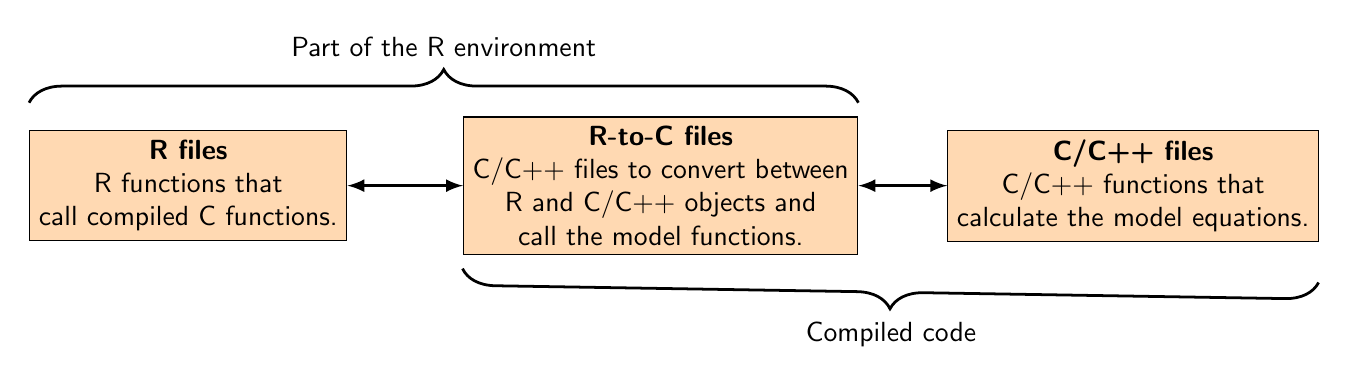
\begin{tikzpicture}[node distance=2 cm, decoration={brace}]
\tikzstyle{process} = [rectangle, minimum width=3 cm, minimum height=1 cm, text centered, draw=black, fill=orange!30]
\node (R)  [process, align=center] {\textbf{R files}\\R functions that\\call compiled C functions.};
\node (RC) [process, align=center, right of=R, xshift=4 cm] {\textbf{R-to-C files}\\C/C++ files to convert between\\R and C/C++ objects and\\call the model functions.};
\node (C)  [process, align=center, right of=RC, xshift=4 cm] {\textbf{C/C++ files}\\C/C++ functions that\\calculate the model equations.};

\draw [latex-latex, line width=1.1 pt] (R) -- (RC);
\draw [latex-latex, line width=1.1 pt] (RC) -- (C);

\draw [decoration={brace, raise=10 pt, amplitude=12 pt}, decorate, line width=1 pt] (R.north west) -- node[above=23 pt] {Part of the R environment} (R.north -| RC.east);
\draw [decoration={brace, raise=10 pt, amplitude=12 pt, mirror}, decorate, line width=1 pt] (R.south -| RC.west) -- node[below=23 pt] {Compiled code} (RC.south -| C.east);

%\draw [decoration={brace, raise=10 pt, amplitude=10 mm}, decorate, line width=1 pt] (R.north west) -- (R.north -| RC.east) {Part} (RC);
%5\draw[decoration={brace, raise=-10 pt, mirror, amplitude=10 mm, raise=5pt},decorate]
%  (RC.north -| RC.west -- node[right=6pt] {$AAAAAAAAAAAAAAAAa$} (C);
  
\end{tikzpicture}
\end{center}
\end{figure}

R code should be written so that it only checks validity of arguments and calls R-to-C functions. R-to-C code should only provide error checking and call C/C++ functions. That is, R and R-to-C functions should only provide a way to access the models written in C/C++, and no modeling should be done in R or R-to-C code.

\subsection{Writing new models}
The C++ code is designed so that the functions have notation similar to the mathematical model. That is, they look like $\frac{dX_{t,cd}}{dt} = h(X_{t})$. In BioCro, functions that implement $h(X_{t})$ are called modules.

As in the R code, both $\frac{dX_{t,cd}}{dt}$ and $X_{t}$ are represented as key-value pairs. The data type used for this in C++ is a \code{state\_map}. As an example, to model leaf growth rate as half of canopy assimilation rate going to leaves, the following code would be used:

\begin{minipage}{\linewidth}
\begin{center}
\begin{lstlisting}[language=c++]
state_map simple_leaf_growth::do_operation(state_map const &s) const
    state_map partial_rates_of_change;
    partial_rates_of_change["Leaf"] = s.at("Assim") * 0.5;
    return partial_rates_of_change;    
}
\end{lstlisting}
\end{center}
\end{minipage}

The function is named \code{do\_operation} and is part of the \code{simple\_leaf\_growth} model. It accepts a \code{state\_map} named \code{s} and returns a \code{state\_map} named \code{partial\_rates\_of\_change}. The current state of the model ($X_t$), is passed in as \code{s}. The \code{const} keywords are required, but do not need to be understood here. Canopy assimilation rate is calculated in a different part of the model, and it is stored in \code{s} with the name \code{Assim}. To access values in a \code{state\_map}, use the \code{at()} function. To assign a value to parameters within a \code{state\_map}, use the \code{[]} operator. Here, half of the assimilation rate is added to the partial rate of change of leaf growth. Note that when called, the code has the same form as $\frac{dX_{t,cd}}{dt} = h(X_{t})$:

\begin{center}
\begin{lstlisting}[language=c++]
rates_of_change = simple_leaf_growth(current_state);  
\end{lstlisting}
\end{center}

A separate module can be written to describe loss of leaf mass. To describe leaf loss as a fraction of the current leaf mass, the following model could be used:

\begin{center}
\begin{lstlisting}[language=c++]
state_map fractional_leaf_loss::do_operation(state_map const &s) const
    state_map partial_rate_of_change;
    partial_rate_of_change["Leaf"] = -s.at["Leaf"] * 0.01;
    return partial_rate_of_change;    
}
\end{lstlisting}
\end{center}

The addition of the partial rates is handled elsewhere in the code, and does not need to be handled when writing new modules. This design allows one to write modules that operate independently, so that one does not need to know how the entire model works in order to modify a specific aspect of the model. To write a new module, one needs to know only what parameters are defined in the state ($X$), which is a relatively short list.

\end{document}

